The terminator T-2000 is a science-fiction spectacle of a robot -- until you see the price. Channeling the inspiration many high school students may have for robotics, MEIOSIS robotics aims to provide an affordable manipulator to educators and enthusiasts. MEIOSIS uses primarily 3-D printed components and easily accessible materials. Among these materials are a Raspberry PI, smart servos and metal tubing. These features create an open-source manipulator accessible to the public to further robotics education.
\hiddensubsection{Physical System Overview}
The physical design of the robotic manipulator will be shown through Figures \emph{\ref{fig:overall}, \ref{fig:base}, \ref{fig:link1},} and \emph{\ref{fig:link2}}.

\begin{figure}[htp]
  \centering
  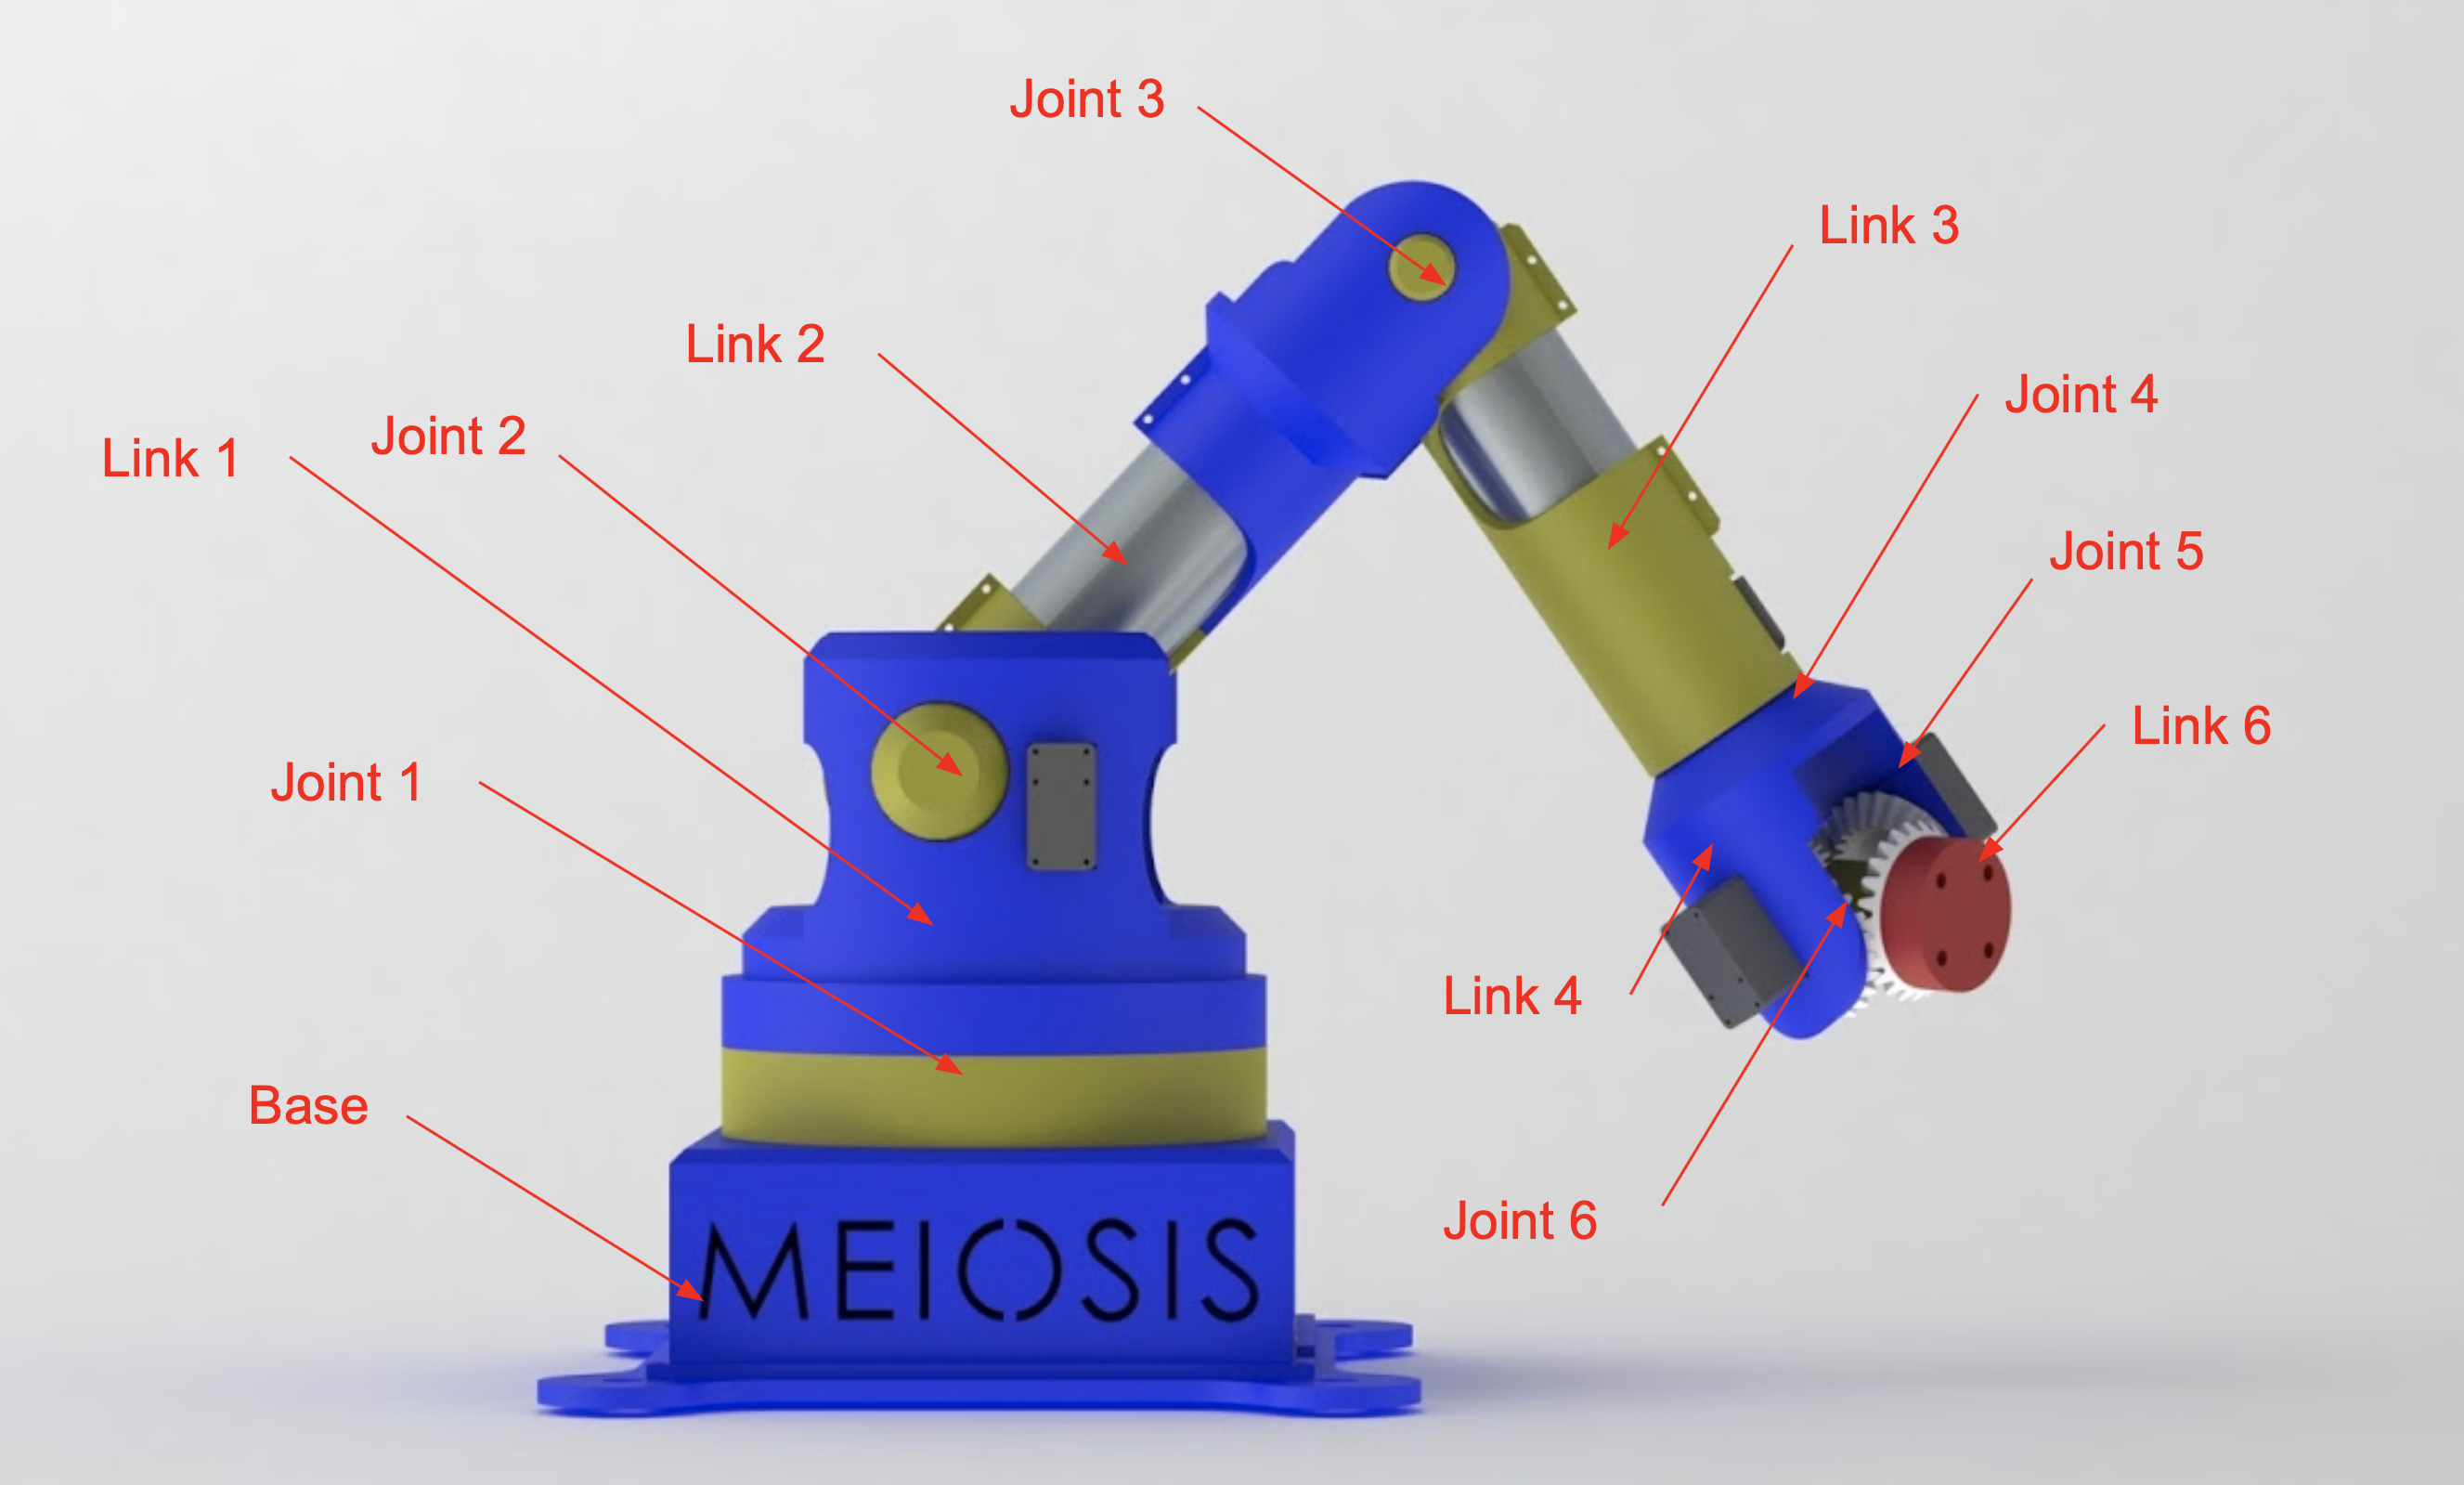
\includegraphics[frame, width=.75\textwidth]{overall_render}
  \caption{Overall System Conceptual Design }
  \label{fig:overall}
\end{figure}

The colored links in \emph{Figure \ref{fig:overall}} distinguish the different joints and links of the manipulator. The overall reach of the robot will be 582.5 mm. This length was chosen to decrease material cost and weight while still satisfying requirement 2.1.2 and 2.1.5, allowing the manipulating to pick and place objects to perform basic tasks. The base of the robot will be made to contain the Raspberry Pi and other electrical components.
\newpage
\subsubsection{Base}
The base of the manipulator will house several of the electronic components, such as the computational system, power supply, and motor controller. A cross section of the base can be seen in \emph{Figure \ref{fig:base}}.
\begin{figure}[htp]
  \centering
  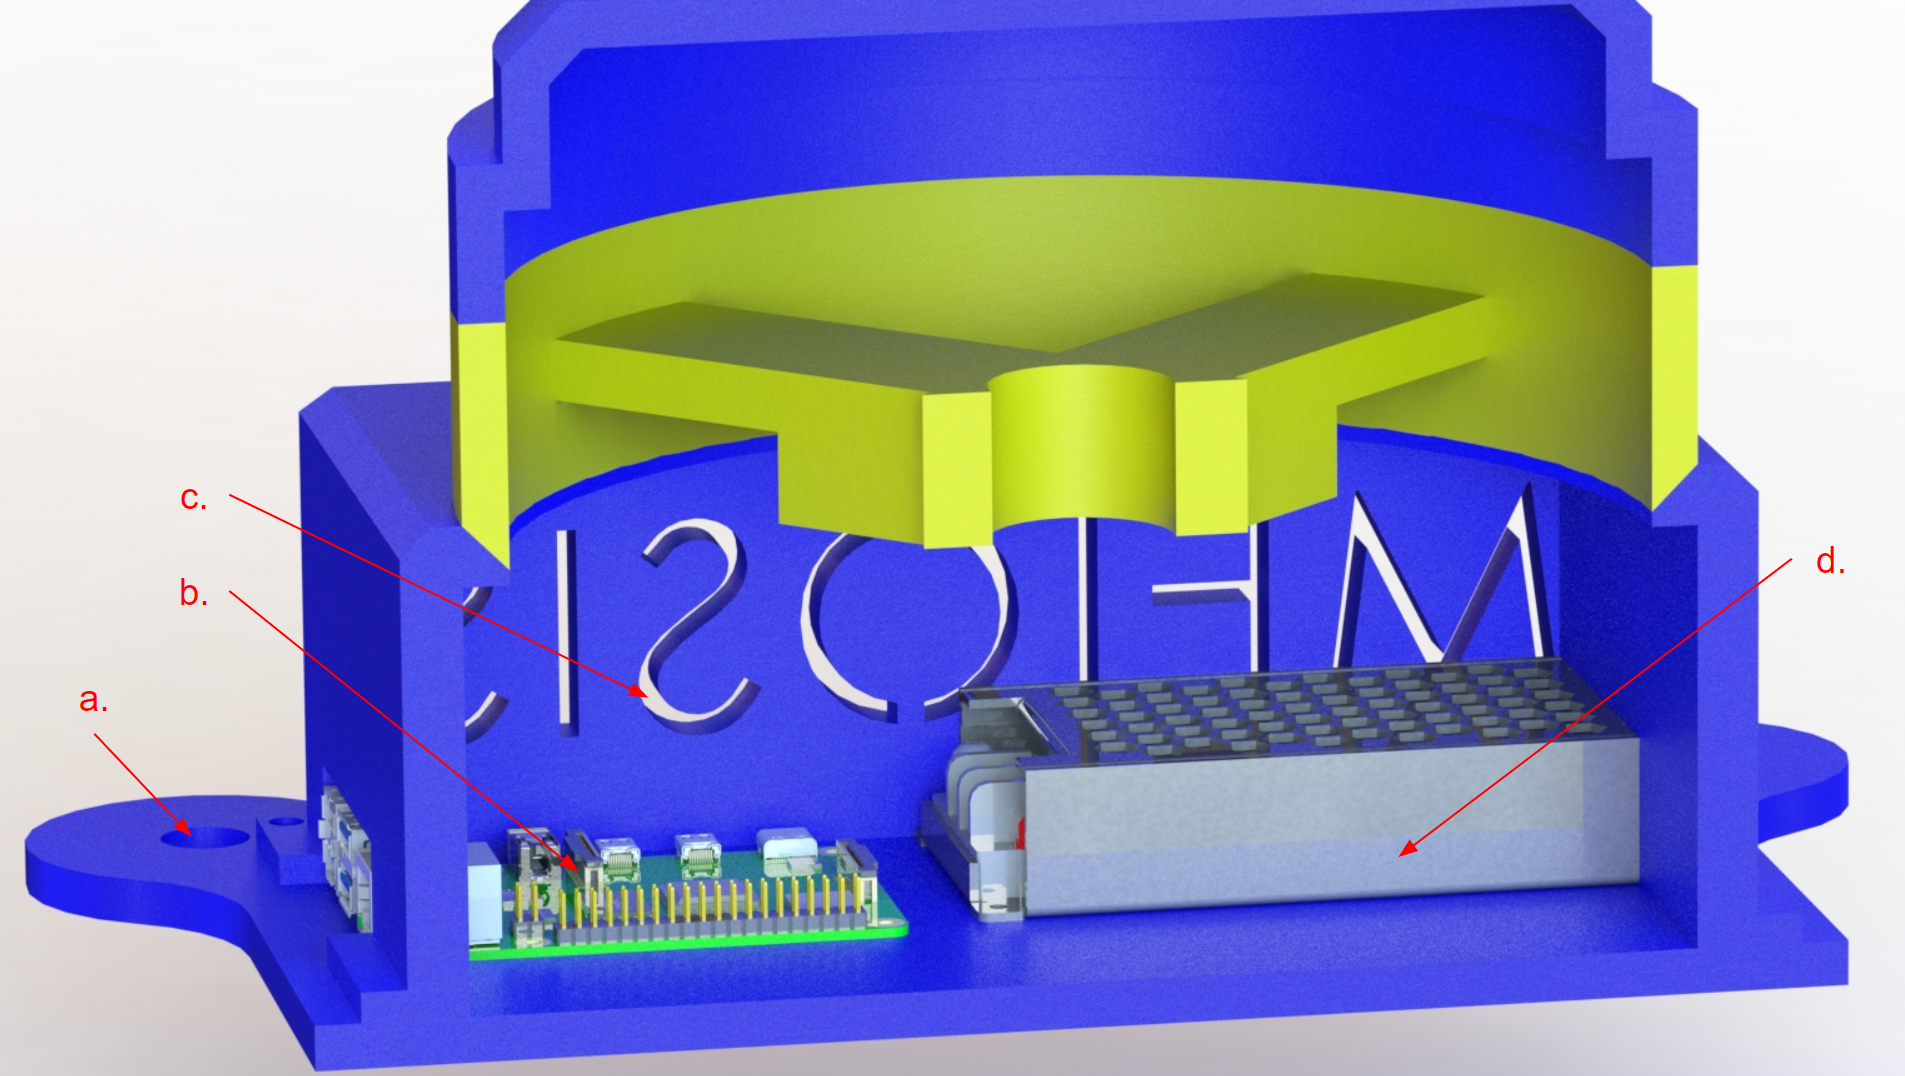
\includegraphics[frame, width=.75\textwidth]{base_callouts}
  \caption{Manipulator Base with Call-outs}
  \label{fig:base}
\end{figure}

From \emph{Figure \ref{fig:base}},
\begin{enumerate}[label=\alph*.]
  \item \emph{Base Supports:}
  The base supports are located at each corner of the base and will allow the base of the manipulator to be securely attached to a variety of surfaces with either standard bolt/fastener hardware or suction cups.
  \item \emph{Computational System:}
  The computational system will be a Raspberry Pi; it will be housed in the base, which allows the Raspberry Pi to be more easily accessible. The primary reason for this system being chosen is to fulfill the budget requirement, 2.1.1. The Raspberry Pi will compute the manipulator's kinematics and command the motors accordingly.
  \item \emph{Airflow Cutouts:}
  The side of the base will have cutouts to allow for airflow through the base; since the power supply is housed inside of the base as well as the computational system, the temperature must be regulated to prevent overheating.
  \item \emph{Power Supply:}
  The power supply will be housed in the base as well; this allows the power supply to be more accessible and therefore more modifiable, so the end-user can easily expand the system to fulfill their needs.
\end{enumerate}
\newpage
\subsubsection{Links}
\emph{Figure \ref{fig:link1}} is an image of the robot that shows the links and their key features.\\
\begin{figure}[htp]
  \centering
  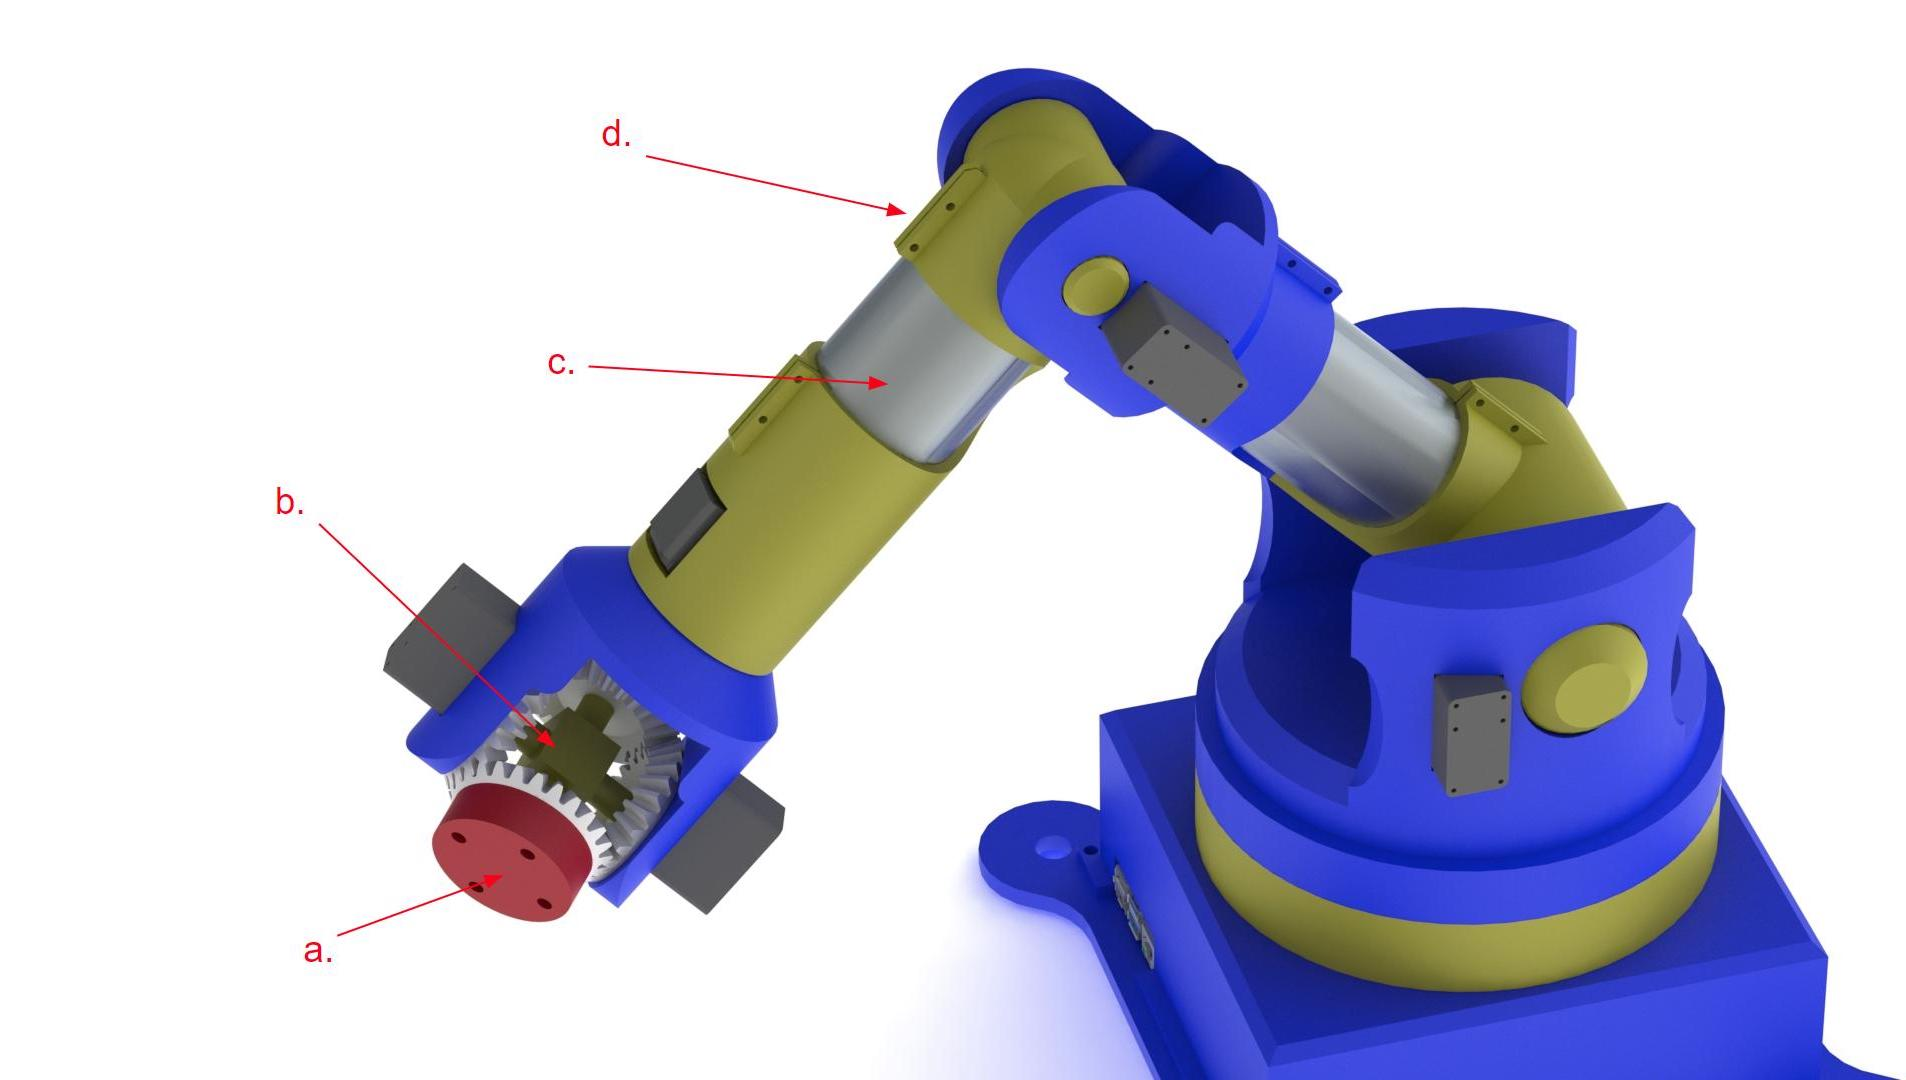
\includegraphics[frame,width=.63\textwidth]{link_callouts}
  \caption{Drawing Showing Key Features of Design}
  \label{fig:link1}
\end{figure} \\
\emph{Figure \ref{fig:link1}} highlights a few of the key features of our design. Call-out a shows the connection point for the end effector. The mountings are the standard used by the Sawyer manipulator. This may be adjusted to accommodate lower cost, more accessible end effectors. Call-out (b) shows the differential gearbox that will be used in the manipulator’s wrist, saving space and weight. The manipulator will have aluminum tubing as support in the links (c) and will be attached to the 3D printed portion of the robot using clamp joints (d) tightened by screws.

\emph{Figure \ref{fig:link2}} is an image of the cross section of link 2 for the manipulator.
\begin{figure}[htp]
  \centering
  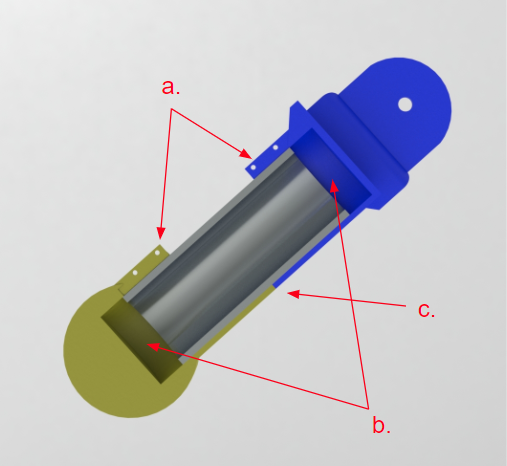
\includegraphics[frame,width=.35\textwidth]{link_cross_section}
  \caption{Drawing Showing Link Cross Section}
  \label{fig:link2}
\end{figure}

The cross section seen in \emph{Figure \ref{fig:link2}} shows the internal design for links two and three. It features two clamps that hold a hollow aluminum bar in place (a) and allows for gaps between the aluminum tube and the 3D printed call-out (b). The proper length will be dictated by the 3D printed guides lining up at call-out (c). This allows for imprecision in the manufacturing of the aluminum tube.

\hiddensubsection{System Functions}
The system can be divided into two subsystems: the electrical and software systems. The electrical subsystem includes the wiring and hardware computational components, power system, actuators with drivers, and sensors. The software subsystem includes the algorithm for the computational system.
\hiddensubsection{Electrical}
\emph{Figure \ref{fig:eblock}} is the block diagram for the electrical system of the manipulator.

\begin{figure}[htp]
  \centering
  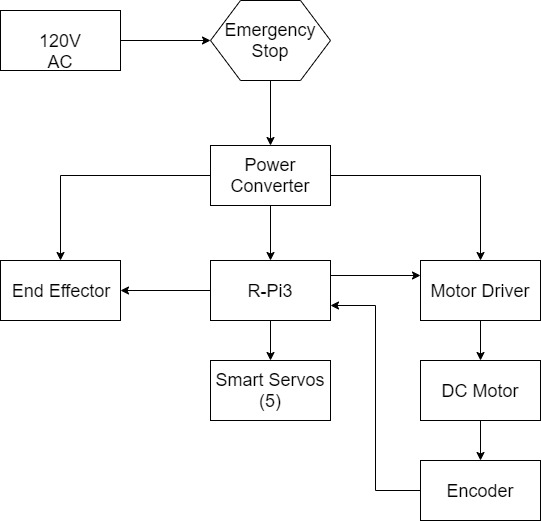
\includegraphics[width=.55\textwidth]{eblock}
  \caption{Electrical System Block Diagram}
  \label{fig:eblock}
\end{figure}

\emph{Figure \ref{fig:eblock}} shows that the electrical systems of the manipulator will be relatively simple. Power is supplied by the 120V AC from standard wall outlets. A power supply will adapt the AC voltage to the required voltages for each component. One component is the Raspberry Pi, which will perform calculations for motor control (described below in software). It will send signals to the DC motor driver and the five smart servos. The smart servos have an on-board controller, so no feedback will be necessary. However, the first joint, between the base and the first link, will be actuated by a DC motor with an encoder to minimize cost.

\hiddensubsection{Software}
\emph{Figure \ref{fig:sblock}} shows the software flowchart for the system.
\begin{figure}[ht]
  \centering
  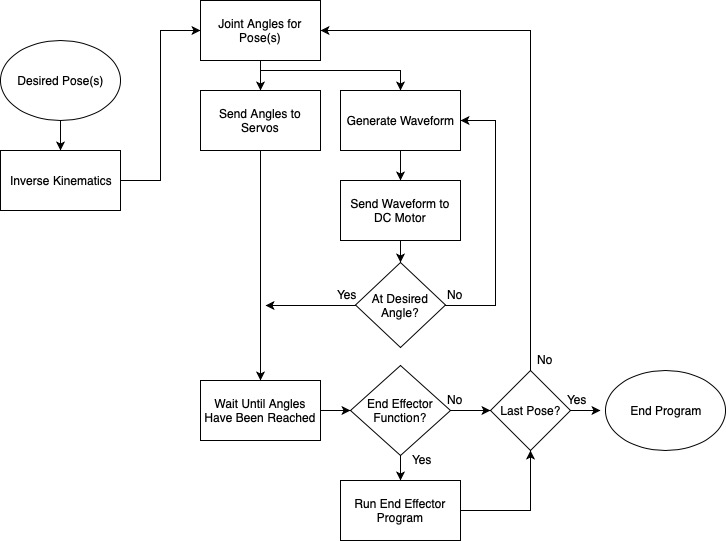
\includegraphics[width=.85\textwidth]{sblock}
  \caption{Software Flowchart}
  \label{fig:sblock}
\end{figure}

Similar to the electrical system, the software is also simple. \emph{Figure \ref{fig:sblock}} shows that the software will receive the desired pose or poses the user would like the manipulator to reach. Then the Raspberry Pi will use inverse kinematics to calculate the necessary joint angles. The wave-forms/desired angles will be sent to the respective drivers/motors, and positional information will be sent back to the Raspberry Pi to adjust the DC motor angle. When the motors have reached their desired pose, the Raspberry Pi will actuate the end effector if it is specified by the user. The system will then check to see if there are any more poses to reach and either repeat the motor control section given the desired angles of the new pose or end program if the last pose has been reached.
